% TEX STUDIO MAGIC-COMMAND
% !TeX document-id = {21ffa6e2-6c8f-4532-897c-386dc477f19a}
% !TeX root = presen.tex
% !TeX encoding = utf8
% !TeX TXS-program:compile = lualatex -synctex=1 -interaction=nonstopmode -halt-on-error %.tex
% !TeX TXS-program:quick = txs:///compile | txs:///view-pdf-internal --embedded
%%%-------------------------------------------------------------------------
%%% PD3プレゼンプレート
%%% 作成: 金沢工大・情報工学科・鷹合研究室
%%%-------------------------------------------------------------------------

% !TeX root = presen.tex
\documentclass[25pt, landscape,oneside]{foils}



% 4:3のスクリーン(古い建物)の場合
%\usepackage[top=15truemm,bottom=22truemm,left=15truemm,right=15truemm,paperwidth=300truemm,paperheight=225truemm]{geometry}

% 16:9のスクリーン(8号館,23号館)の場合
\usepackage[top=15truemm,bottom=22truemm,left=15truemm,right=15truemm,paperwidth=320truemm,paperheight=180truemm]{geometry}


% 箇条書き環境の余白設定
\usepackage[shortlabels]{enumitem}
\setlist[description]{topsep=3mm,parsep=0mm,partopsep=0mm,itemsep=.5\zh,leftmargin=2\zw,labelsep=.5\zw}
\setlist[enumerate]{topsep=3mm,parsep=0mm,partopsep=0mm,itemsep=.5\zh,leftmargin=2\zw,labelsep=.5\zw}
\setlist[itemize]{topsep=3mm,parsep=0mm,partopsep=0mm,itemsep=.5\zh,leftmargin=2\zw,labelsep=.5\zw}


%%%%%%%%%%%%%%%%%%
% フォントの設定
%%%%%%%%%%%%%%%%%%
\usepackage[no-math,deluxe,expert,haranoaji]{luatexja-preset}

\iftrue % 全体的に細身のフォントが良いとき
%\iffalse  % 太めのフォントが良いとき
\setmainfont[BoldFont=HaranoAjiMincho-Bold]{HaranoAjiMincho-Light}
\setsansfont[BoldFont=HaranoAjiGothic-Medium]{HaranoAjiGothic-Light}
\setmainjfont[BoldFont=HaranoAjiMincho-Bold]{HaranoAjiMincho-Light}
\setsansjfont[BoldFont=HaranoAjiGothic-Medium]{HaranoAjiGothic-Light}
\else
\setmainfont[BoldFont=HaranoAjiMincho-Bold]{HaranoAjiMincho-Regular}
\setsansfont[BoldFont=HaranoAjiGothic-Bold]{HaranoAjiGothic-Regular}
\setmainjfont[BoldFont=HaranoAjiMincho-Bold]{HaranoAjiMincho-Regular}
\setsansjfont[BoldFont=HaranoAjiGothic-Bold]{HaranoAjiGothic-Regular}
\fi

\setmonofont{Inconsolata}  % urlやverbatim,listingsなどの欧文フォント

\renewcommand{\kanjifamilydefault}{\gtdefault}  % 日本語フォントをゴシックに
\renewcommand*\familydefault{\sfdefault}
%\mathversion{bold} % 数式フォントを太字に変更する

\usepackage{alltt,upquote,textcomp} % シングル,バッククォートなどの視認性をアップ!
\def\textasciigrave{\char0}

% このパッケージを入れないと verbatim の日本語が何故かゴシックにならない
\usepackage{verbatim}% 


%%%%%%%%%%%%%%%%%%
% PDFの設定
%%%%%%%%%%%%%%%%%%

\usepackage[%
pdfstartview={FitH -32768},%    描画領域の幅に合わせる
bookmarks=true,%                しおり付き
bookmarksnumbered=true,%        章や節の番号をふる
bookmarkstype=toc,%             目次情報のファイル.tocを参照
colorlinks=true,%              ハイパーリンクを色枠に
linkcolor=black,%
urlcolor=black,%
citecolor=black,%
filecolor=black,%
menucolor=black,%
pagecolor=black,%
pdftitle={プロジェクトデザイン3},
pdfsubject={},
pdfauthor={鷹合研究室},
pdfkeywords={},
dvipdfmx-outline-open %%%%%%%%%%%%%%% これがあるとBookmarkを自動的に展開されるみたい・・・
]{hyperref}


%%%%%%%%%%%%%%%%%%%%%%%%%%%
%
% ここから下は必要がない限り書き換えない
%
%%%%%%%%%%%%%%%%%%%%%%%%%%

%%%%%%%%%%%% ブックマークを表示
\usepackage{bookmark}

% スライドの見出しの位置
\setlength{\foilheadskip}{-14mm}

% スライドなので字下げしない
\setlength{\parindent}{0mm}


% ルビ
\usepackage{luatexja-ruby}

\usepackage{bbding} % \PencilRightDown 鉛筆マーク
\usepackage{tikz}
\usepackage[symbol]{footmisc}
\usepackage{xcolor,listings}
\usepackage{multicol}
\usepackage{xurl}
\usepackage{graphicx}
\usepackage{epsfig}

\usepackage{lastpage}
\usepackage{ascmac}
%\usepackage{fancybox,fancyvrb,okumacro}

\renewcommand{\lstlistingname}{List} 

\lstset{%
	language={Python}, 
	backgroundcolor={\color[gray]{.95}},%
	basicstyle={\ttfamily\small},%
	identifierstyle={\ttfamily\small},
	commentstyle={\ttfamily\small\color{red}},
	keywordstyle={\ttfamily\small\color{blue}},
	ndkeywordstyle={},%
	stringstyle={\ttfamily\small\color[rgb]{0,0.5,0}},
	frame={tb},
	breaklines=true,
	columns=[l]{fullflexible},
	%	columns=[l]{fixed},% fixed だと開きすぎ
	basewidth=0.5em,   % これないと行頭のスペースが揃わない
	numbers=left,%
	xrightmargin=0\zw,%
	xleftmargin=3\zw,%
	numberstyle={\ttfamily\small},%
	tabsize=3,
	stepnumber=1, 
	numbersep=0.75\zw,%
	lineskip=-0.3ex,%
	belowcaptionskip=3pt,   % これないと見出しとリスト本体に隙間が毎回変わる
	abovecaptionskip=0pt,
	captionpos=t,
	showstringspaces=false, % 半角スペースを記号で表示しない
}
%

%%%%%%%%%%%% fboxの線幅
\setlength{\fboxrule}{1.5pt}



%%%%%%%%%%%% ページフッタの設定 %%%%%%%%%%%%%
\usepackage{fancyhdr}
\pagestyle{fancy}
\fancyhf{}  % これを入れないと2ページのフッタがずれる
\renewcommand{\headrulewidth}{0pt} % 水平線を消去
\renewcommand{\footrulewidth}{0pt} % 水平線を消去
\renewcommand{\thefootnote}{\fnsymbol{footnote}}

%%%%%%%%%%%%%%%%%%%%%%%%%%%%%%%%%%%%%%
% Verbatim環境にデフォルト値をセット
\usepackage{fancyvrb}
\newenvironment{verbatimx}%
{\small\Verbatim[frame=single,obeytabs,baselinestretch=.65,commandchars=\\\{\}]}%
{\endVerbatim}%

%%%%%%%%%%%%%%%%%%%%%%%%%%%%%%%%%%%%%%
% Verbatim環境にデフォルト値をセット
\newenvironment{myVerbatim}%
{\vspace{-8mm}\Verbatim[frame=single,obeytabs,framesep=2mm,baselinestretch=.7,commandchars=\\\{\}]}%
{\endVerbatim}%


%%%%%%%%%%%%%%%%%%%%%%%%%%%%%%%%%%%%%%
\usepackage{fontawesome5}
\renewcommand{\refname}{文献} % 文献の表記を変更

%%%%%%%%%%%%%%%%%%%%%%%%%%%%%%%%%%%%%%%%%
\renewcommand{\lstlistingname}{リスト}

% 図・表・リストのcaption番号を表示するか/表示しないかを選ぶ
\iffalse
\usepackage[hang,bf,labelformat = empty,labelsep=none,figurename=Y, tablename=X, singlelinecheck=off,justification=centering,labelfont=bf,textfont=bf]{caption} 
\else
\usepackage[hang,bf,labelsep=colon,figurename=図, tablename=表, singlelinecheck=off,justification=centering,labelfont=bf,textfont=bf]{caption} 
\fi

%%%%%%%%%%%%%%%%%%%%%%%%%%%%%%%%%%%%%%%%%
% 
% タイトルスライドのロゴ画像
% フッタ(左)
%%%%%%%%%%%%%%%%%%%%%%%%%%%%%%%%%%%%%%%%%
%  フッタ(左側)

  \MyLogo{
\includegraphics[height=1.1cm]{fig/logo/kit_landscape1.pdf}}
% \MyLogo{--- 鷹合研究室 ---} % トップスライドの下部中央

  \lfoot{
\includegraphics[height=.75cm]{fig/logo/kit_landscape1.pdf}}
% \lfoot{\small 鷹合研}        % フッタ(左)

%%%%%%%%%%%%%%%%%%%%%%%%%%%%%%%%%%%%%%%%%
% 
% フッタ(中央,右)
%
%%%%%%%%%%%%%%%%%%%%%%%%%%%%%%%%%%%%%%%%%
%\cfoot{\thepage/\pageref{LastPage}} 
\cfoot{\thepage/\pageref{LastPage}}
\rfoot{\small 4EP404} % テーマ番号

%%%%%%%%%%%%%%%%%%%%%%%%%%%%%%%%%%%%%%%%%%%
% ページ番号を1からにしたら,トップスライドの下部のロゴがうまくいかなくなったのでこうしてみた
\fancypagestyle{myfirstpage}
{
  \fancyhf{}
   \fancyfoot[C]{
\includegraphics[height=1.1cm]{fig/logo/kit_landscape1.pdf}}
%  \fancyfoot[C]{鷹合研究室}
   \renewcommand{\headrulewidth}{0pt} % removes horizontal header line
}
%%


%%%%%%%%%%%%%%%%%%%%%%%%%%%%%%%%%%%%%%%%%
% 
% ここから下を書き換えて下さい 
%
%%%%%%%%%%%%%%%%%%%%%%%%%%%%%%%%%%%%%%%%%

\title{
{\normalsize 令和6年度 プロジェクトデザインIII}\\\vspace{10mm}
{\LARGE WebAssemblyを用いた\\グラフィクスレンダリングの高速化}
}
\date{令和6年09月25日}
\author{
4EP4-04\\ \ruby{天羽}{あもう}\ruby{大樹}{たいき}
}



\begin{document}
\maketitle % タイトルページ
\addtocounter{page}{1}
\thispagestyle{myfirstpage}

%%%%%%%%%%%%%%%%%%%%%%%%%%%%%
 \foilhead{\Large 1. はじめに -- 背景と目的 -- }
\begin{itemize}
 \item 将来、Webアプリケーションとして、リアルタイムに変化するxRコンテンツを作成し、動作させる際、グラフィクスレンダリングの速度が遅くなってしまうと、没入感を損なってしまう問題があると考えられる
 \item そのような問題に対処するために、Webブラウザ上でグラフィクスのレンダリングを早く処理するために、どのような手法を用いれば、より早く処理できるのかという取り組みを行う必要がある
 \item 本プロジェクトにおいては、WebAssemblyという仕組みを用いたバイナリフォーマットプログラムを使って、グラフィクスレンダリングを早く処理させるプログラムを作成する
\end{itemize}
\newpage

%%%%%%%%%%%%%%%%%%%%%%%%%%%%%
\foilhead{\Large 発表の流れ}
\begin{enumerate}[itemsep=0.25\zh]
	\item \textcolor{gray}{はじめに -- 背景と目的 --}
	\item \textcolor{red}{用語などの簡潔な説明}
	\item プログラム概要
	\item 性能比較評価・考察
	\item むすび
\end{enumerate}
\newpage

%%%%%%%%%%%%%%%%%%%%%%%%%%%%%%%%%%%%%%%%%%%%%%
\foilhead{\Large 2. 用語の簡潔な説明}
\begin{itemize}
	\item WebAssembly\\Webブラウザに搭載されている仮想マシンで\\実行できるバイナリコードとそれを処理するシステム全体\cite{WebAssembly}のこと。\\wasmと略して呼称されることが多いため、本スライドでも\\その略称を以後使用する。特定のプログラミング言語で記述した\\プログラムをそのバイナリコードにコンパイルしたものを\\主に指す。そのプログラムを保存したファイルは、\\wasmモジュールと呼称されることが多い。\\C,C++,Rustなどで記述したプログラムをこのWebAssemblyに\\コンパイルすることで、動作させることが可能になる。\cite{FromCompileLang}
	\newpage
	
	
	\item WebGPU\\WebGLより高度にGPUの性能を活かし、高速なグラフィクス\\レンダリングを行うことが可能であるとされている\\ブラウザ組み込みのAPI。まだ公開されてから日が浅いため、\\著名な関連ライブラリなどはまだあまり見受けられない
\end{itemize}
\newpage

\foilhead{\Large 2-1. なぜWebAseemblyを扱うのか}
\begin{description}
	\item[扱うメリット]~\\
	WebAssemblyはWebブラウザ上でネイティブコードに近い速度で実行される\cite{WasmLikeNativeSpeed}ため、JavaScriptでは時間がかかるであろう処理をWebAssemblyでの処理に置き替えることによる高速化が望める
	\item[WebAssemblyが得意とする処理]~\\
	基本的に、WebAssemblyそのものは、整数・実数の計算しかできない\cite{WasmOnlyCalc}が、WebAssemblyが既にコンパイルされた仮想マシンコードであることを活かし、高速な演算処理を得意とする。	
\end{description}
\newpage
%%%%%%%%%%%%%%%%%%%%%%%%%%%%%
\foilhead{\Large 発表の流れ}
\begin{enumerate}[itemsep=0.25\zh]
	\item \textcolor{gray}{はじめに -- 背景と目的 --}
	\item \textcolor{gray}{用語などの簡潔な説明}
	\item \textcolor{red}{プログラム概要}
	\item 性能比較評価・考察
	\item むすび
\end{enumerate}
\newpage

%%%%%%%%%%%%%%%%%%%%%%%%%%%%%%%%%%%%%%%%%%%%%%

\foilhead{\Large 3. プログラム概要}
Rustでブラウザに搭載されているAPIにアクセスするプログラムを記述し、\\そのプログラムをWebAssemblyにコンパイルする。\\コンパイルされたプログラムをJavaScriptでロードし、実行させる。\\
WebAssembly側で処理するプログラムの対象として、
\begin{itemize}
	\item 比較的、ハードウェア側に近いプログラムの処理
	\item 行列などを扱う演算負荷の高い処理
\end{itemize}
というような処理を指定して行う

%% \begin{figure}[h]
%% \begin{center}
%% 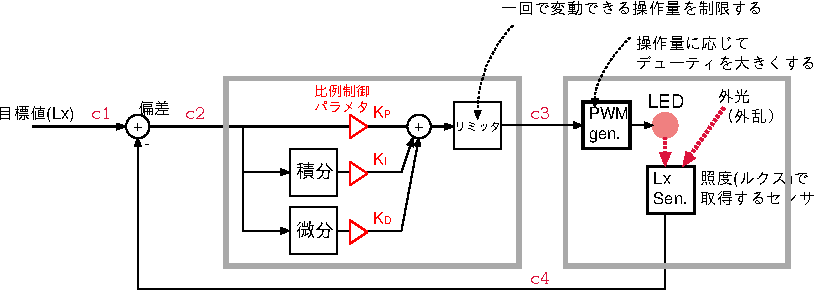
\includegraphics[width=\textwidth]{fig/system.pdf}
%% \caption{}
%% \end{center}
%% \end{figure}
\newpage

%%%%%%%%%%%%%%% minipage の利用例 %%%%%%%%%%%%%%%%%%%
%------ 左側
\begin{minipage}[t]{0.4\textwidth}\vspace{0pt}
本プロジェクトでは、2つの\\プログラミング言語を用いて\\高速化を行う

\begin{enumerate}[parsep=-0.5\zh]
	\item Rustのプログラムで\\グラフィクスを操作するAPIをコール
	\item Rustのプログラムを\\WebAssemblyに\\コンパイルする
	\item WebAssemblyプログラムをJavaScript側から\\コールする
\end{enumerate}
\end{minipage}
%------ 右側
\begin{minipage}[t]{0.6\textwidth}\vspace{0pt}
\begin{center}
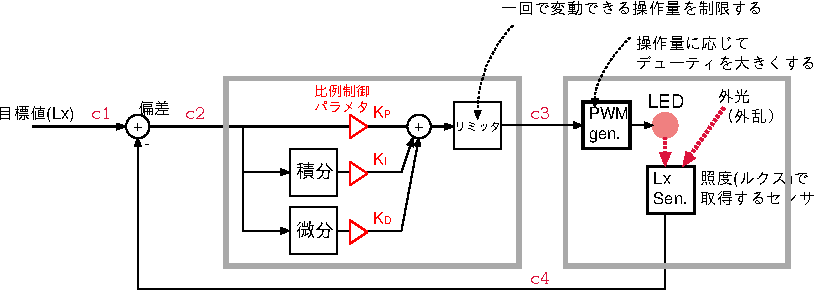
\includegraphics[keepaspectratio, width=.9\linewidth,trim={0mm 0mm 0mm 0mm},clip]{fig/system.pdf}
\end{center}
\end{minipage}

%%%%%%%%%%%%%%%%%%%%%%%%%%%%%%%%%%%%%%%%%%%%%%
\foilhead{\Large 3-1. 作成したWebAssemblyプログラムの概要}
\begin{description}

	\item[処理内容]~\\
	WebGPU APIを通してレンダリング内容を決め、実行する内容をバッファデータとして処理し、順番に実行させる一連の処理を行う
	\item[実行される処理の結果]~\\
	HTMLのcanvas要素の範囲にプログラムで指定した\\矩形や図形がレンダリングされる

\end{description}
\newpage

%%%%%%%%%%%%%%%%%%%%%%%%%%%%%
\foilhead{\Large 発表の流れ}
\begin{enumerate}[itemsep=0.25\zh]
	\item \textcolor{gray}{はじめに -- 背景と目的 --}
	\item \textcolor{gray}{用語などの簡潔な説明}
	\item \textcolor{gray}{プログラム概要}
	\item \textcolor{red}{性能比較評価・考察}
	\item むすび
\end{enumerate}
\newpage

%%%%%%%%%%%%%%%%%%%%%%%%%%%%%%%%%%%%%%%%%%%%%%
\foilhead{\Large 4. 性能比較評価・考察}

\begin{description}
	
	\item[評価方法とその手順]~\\
	次ページの画像のような色の異なる三角形をそれぞれレンダリングする際、JavaScriptのみで組んだ関数と、WebAssemblyを交えたプログラムを同時に実行しその2つの関数の実行が終了するまでの時間を\\JavaScriptのperformanceクラスのメソッドを利用して、\\実行を終了した時間から実行を開始した時間を減算することで計測。\\
	これを、for文で500回行った実行時間データをCSVデータとし、Python言語を用いて平均値、中央値、最大値、最小値を算出する。
	また、Pythonライブラリである、\textbf{matplotlib.pyplot}を使用し、箱ひげ図を作成することにより、安定的に高速化が可能かどうかを評価する
	\newpage
	\begin{figure}[h]
		\centering
		\begin{minipage}[b]{0.38\columnwidth}
			\centering
			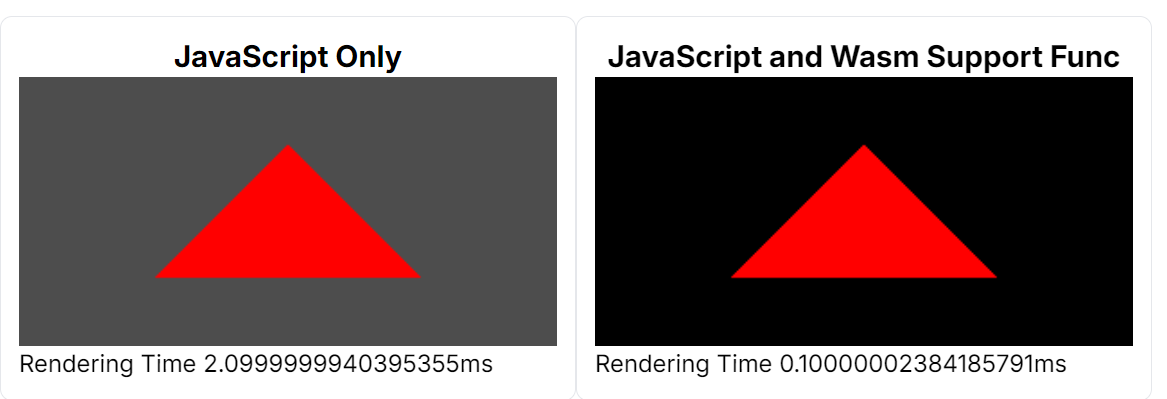
\includegraphics[width=0.9\columnwidth]{normal_triangle.png}
			\label{fig:a}
		\end{minipage}
		\begin{minipage}[b]{0.38\columnwidth}
			\centering
			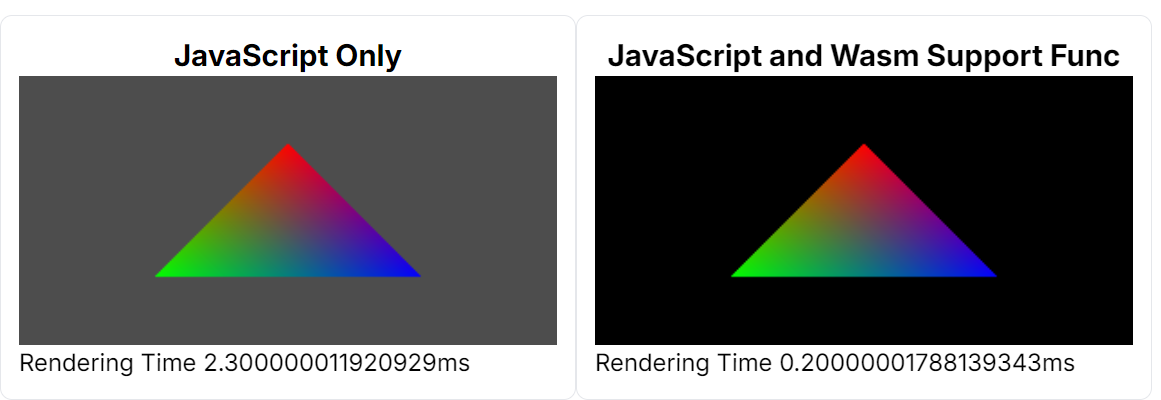
\includegraphics[width=0.9\columnwidth]{colorful_triangle.png}
			\label{fig:b}
		\end{minipage}
	\end{figure}
	\begin{description}
		\item[比較対象に関する詳細な説明]~\\	
		比較対象は、描画プログラムを以下のように記述したものである。
		\begin{itemize}
			\item 左画像の左側が、JavaScriptのみで記述したもの
			\item
			左画像の右側が、JavaScript+Wasmで記述したもの
			\item
			右画像の左側が、JavaScriptのみでカラフルな図形を\\レンダリングするように記述したもの
			\item
			右画像の右側が、JavaScrpt+Wasmでカラフルな図形を\\レンダリングするように記述したもの
		\end{itemize}	
	\end{description}
	\newpage
	
	\item[評価結果]~\\
	以下の表には、計算した4つの値について記載する。\\
	時間の単位については全てミリ秒である。
	
	\begin{table}
	\begin{tabular}{|c|c|r|r|r|r|} \hline
		描画内容&Wasmの有無&平均時間&最小時間&最大時間&時間の中央値\\
		赤色三角形&無&0.445691&0.1&2.0&0.4\\
		赤色三角形&有&0.424649&0.1&1.6&0.4\\
		虹色三角形&無&0.413427&0.1&1.7&0.4\\
		虹色三角形&有& 0.416232&0.1&1.9&0.4\\ \hline
	\end{tabular}
	\end{table}
	
	%今回の比較では、以下の結果が出た。このケースではそれほど大きな差が出なかった。\\
	% また、今回は単一の図形のレンダリングのみなので、映像ではなく画像でレンダリング時の画面を掲示する。
	
	\newpage
	\begin{minipage}[t]{0.4\textwidth}\vspace{0pt}
		右記の箱ひげグラフの結果から、以下のようなことが言える
		
		\begin{enumerate}[parsep=-0.5\zh]
			\item 箱ひげ自体に着目すると、大きな変化があるようには見受けられない
			\item 赤色の図形は最遅の場合の時間が短縮されているが、それ以外の目立った違いが見受けられない
			\item 虹色のもの場合は、最遅のケースを比較した際、実行時間が増えてしまっている。
		\end{enumerate}
	\end{minipage}
	%------ 右側
	\begin{minipage}[t]{0.6\textwidth}\vspace{0pt}
		\begin{center}
			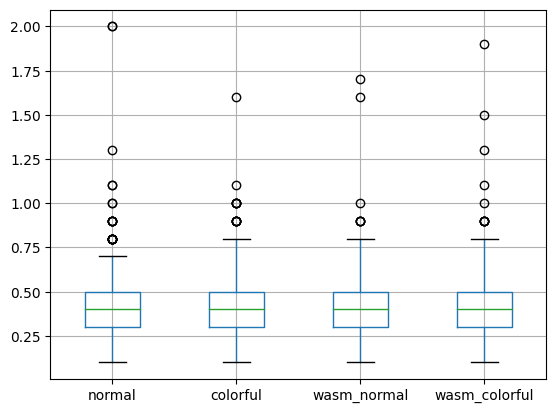
\includegraphics[keepaspectratio, width=.9\linewidth,trim={0mm 0mm 0mm 0mm},clip]{box_chart.png}
		\end{center}
	\end{minipage}
	\newpage
	\item[考察]~\\
	% 今回は単純な単色の図形、もしくは三色のグラデーションの図形のみ\\の描画であるため、大きな差にはならなかったと考えられる。\\しかし、2つの比較で、色のグラデーションを持つ三角形の方が\\高い速度差を示しているため、色の演算処理が増えた分の差が\\出ていると考えられる。そのため、より内部の数値処理を増やすと、\\より大きな差が生まれる可能性があると考えられる
	\begin{description}
		\item[赤色三角形の場合]~\\
		平均値や最大値のデータやグラフからは、単純かつ単色の図形のレンダリングであれば、高速化が見込める可能性があるといえる
		\item[虹色三角形の場合]~\\
		虹色三角形の場合は、平均値や最大値のデータやグラフから、\\むしろ遅くなってしまっていることがわかる。
		\item[結果から]~\\
		矩形自体のレンダリングに関しては高速化が可能であると考えられるが、
		色の複雑な処理が入ってしまうと、むしろ減速してしまうため、
		カラフルな描画対象を扱う状況にには不向きであると考えられる
	\end{description}

	
\end{description}

% 	\item このスライドでは何をどのような方法で評価したかを明記し,結果をグラフで示すこと(表よりグラフのほうが良い).
%	\item システムが動いている様子がわかるようにデモ映像を流すこと(デモ映像には字幕をつけたりするなどしてわかりやすくすること).
%	\item 評価の際は,改良の前後でどうなったかを示す.あるいは他の手法などと比較してどうなのかを示すことも必要.
%	\item 結果について考察も示すこと.

\newpage

%%%%%%%%%%%%%%%%%%%%%%%%%%%%%%%%%%%%%%%%%%%%%%
\foilhead{\Large 5. むすび}\label{MUSUBI}
\begin{itemize}
	\item Web上でのグラフィクスレンダリングを高速化するため、WebAssemblyを用いたモジュールを作成した。
	\item 現時点では、1つの図形しか描画していないため、それほど大きな描画速度の差がないが、描画物を増やしたらどう変化するのかを検証しようと考えている。
	\item 来月の報告までに、図形の量を増やすことや、プログラム内容の質を高め、より負荷が高くなるプログラムで比較を行う
\end{itemize}
\newpage

%%%%%%%%%%%%%%%%%%%%%%%%%%%%%% 参考文献 %%%%%%%%%%%%%%%%%%%%%%%%%%%%%%
\begin{thebibliography}{99}
\small
\setlength\itemsep{-0.5\zh}%
\bibitem{WebAssembly}日向俊二. (2021). より速く強力なWebアプリ実現のためのWebAssemblyガイドブック (初). カットシステム.
\bibitem{FromCompileLang}[1]と同様
\bibitem{WasmLikeNativeSpeed}Gallant, G. (2022). ハンズオンWebAssembly ──EmscriptenとC++を使って学ぶWebAssemblyアプリケーションの開発方法 (初). オライリー・ジャパン.
\bibitem{WasmOnlyCalc}[1]と同様
%\bibitem{book1} K.Thompson,D.M.Ritchie,\textbf{"The UNIX Time-Sharing System"},Communications of the ACM, Vol.17, No.7, 1974.
%\bibitem{book4} Digital Equipment Corporation: \textbf{PDP11/20-15-r20 Processor Handbook}, 1971.
%\bibitem{Preliminary} T.R. Bashkow, \textbf{"Study of UNIX: Preliminary Release of Unix Implementation Document"}, \url{ http://minnie.tuhs.org/Archive/Distributions/Research/Dennis_v1/PreliminaryUnixImplementationDocument_Jun72.pdf}, Jun. 1972.
%\bibitem{book2} K. Thompson,D.M. Ritchie,"UNIX PROGRAMER'S MANUAL",Nov. 1971.
%\bibitem{web0} Warren Toomey, "The Unix Heritage Society", \url{https://www.tuhs.org/}, Dec. 2015.
% \bibitem{simh} simh, \textbf{"The Computer History Simulation Project"}, \url{https://github.com/simh/simh}, 参照Mar.14, 2022.
% \bibitem{ref0} W.Toomey, \textbf{"First Edition Unix: Its Creation and Restoration"}, IEEE Annals of the History of Computing, 32 (3), pp.74-82, 2010.
%\bibitem{web1} Jim Huang, "Restoration of 1st Edition UNIX from Bell Laboratories", \url{https://github.com/jserv/unix-v1}, 参照Mar.14, 2022.
% \bibitem{book3} Diomidis.Spinellis,\textbf{"unix-history-repo"},  \url{https://github.com/dspinellis/unix-history-repo/tree/Research-V1}, 参照Mar.14, 2022.
% \bibitem{book5} Digital Equipment Copporation: \textbf{PDP11 Peripherals HandBook}, 1972.
%\bibitem{book6} \url{https://github.com/No000/unix-v1-utils}
%\bibitem{book7} \url{https://github.com/No000/UnixV1-SystemCallTracer}
\end{thebibliography}

\end{document} 
